\section{Stability of the 2-body System using Runge-Kutta and Velocity-Verlet}
\label{sec:stability2bodysystem}
The considered two-body system consists of an Earth-like body that orbits a Sun-like body at an initial distance of 1 AU. 
The initial velocity is chosen so that the orbital period of the Earth-like body is 365 days, and due to the choice of the initial position of the Earth-like body relative to the Sun-like body and the initial direction of the velocity of the Earth-like body, the orbit of the Earth-like body is purely in the $x-y$-plane.
Two cases are considered: the situation when the Sun is at rest compared to the frame of reference at all times, and the situation with both the Sun and the Earth moving relative to the frame of reference.
The chosen position and velocity vectors for the Earth and Sun in these two situations are shown in \tabref{tab:SunEarthMarsTest}. 
\begin{table}[H]
\centering
\caption{
Initial position and velocity for Earth and Sun in the Sun-Earth-like two-body system. 
F1 refers to the frame of reference at which the Sun is at rest in origo at all times, whilst F2 refers to the frame of reference in which both the Sun and the Earth moves relative to the coordinate axis. 
The mass of the Earth is given in solar masses, that is $\textrm{M}_E = 3.0\times 10^{-6} \textrm{M}_{\odot}$, and the gravitational constant is given is $2.96\cdot 10^{-4} \frac{\textrm{AU}^2}{\textrm{days}^2 \textrm{M}_{\odot}}$ (see \secref{sec:Conversion}).
}
\begin{center}
\begin{tabular}{ | c | c | c |  }
  \hline			
   &  $\v{r}_{initial}$ [AU] & $\v{v}_{initial}$ [AU/day]  
  \\ \hline
  Earth (F1) & $(1.0,0.0,0.0)$ & $(0.0,0.017,0.0)$
  \\ \hline
  Sun (F2) & $(1.0,1.0,1.0)$  & $(0.0,0.0,0.0)$ 
  \\ \hline
  Earth (F2)  & $(2.0,1.0,1.0)$ & $(0.0,0.017,0.0)$
  \\ \hline
\end{tabular}
\end{center}
\label{tab:SunEarthMarsTest}
\end{table}
\figref{fig:SunEarthMarsTest} shows the final distance between the two bodies as a function of time step length for the two situations: one in which sun is stationary relative to frame of reference and another in which sun is moving relative to the frame of reference. 
In both cases the final distance after 100 years is calculated between the Sun- and the Earth-like bodies and plotted as a function of length of time steps using both the fourth order Runga Kutta method and the Velocity-Verlet method. 
\begin{figure}[H]
\centering
\begin{minipage}{.5\textwidth}
  \centering
  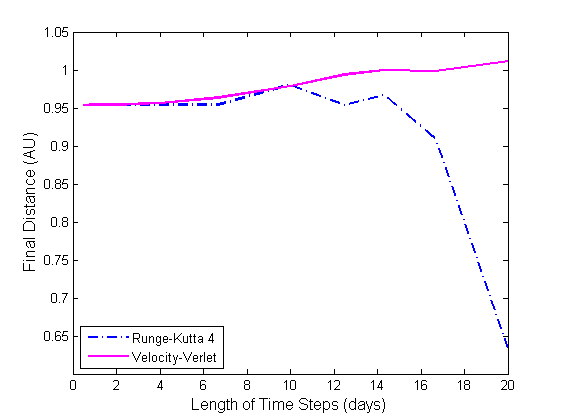
\includegraphics[width=1\linewidth]{Figures/Test_2body_system_earth.png}
\end{minipage}%
\begin{minipage}{.5\textwidth}
  \centering
  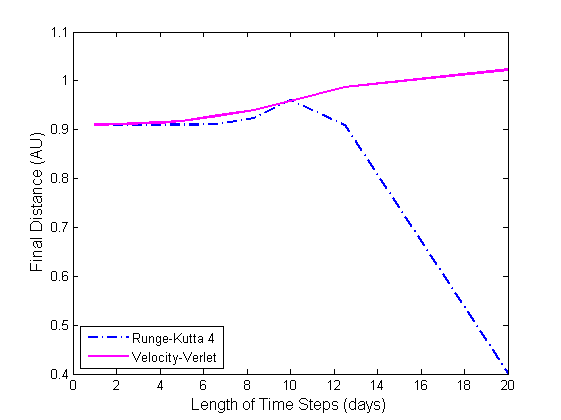
\includegraphics[width=1\linewidth]{Figures/Test_2body_system_earth_sun.png}
\end{minipage}
\caption{
Distance between bodies after 100 years as a function of time step length for the Earth-Sun-like two-body system using both the forth order Runge-Kutta method and the Velocity-Verlet method. 
The leftmost plot do not allow for Sun motion relative to the frame of reference, whilst the rightmost allows for movement of both the Earth and the Sun relative to the frame of reference.
}
\label{fig:SunEarthMarsTest}
\end{figure}
The result using the Velocity-Verlet method shows a gradual increase in the final distance between the two bodies after 100 years, as the length of time steps increases, whereas the final distance after 100 years gained by the fourth order Runga-Kutta method shows fluctuations for shorter time step lengths, which is slightly more when sun is stationary relative to the frame of reference.
As time step length reaches about 10 days, the distance, determined by the Runge-Kutta method, between the two bodies decreases, and the final distance after 100 years between the Earth-like body and the Sun-like body starts varying a lot with a change in time step length, meaning that the Runge-Kutta method is very unstable for large time steps, greater than approximately 10 days for this situation.
However, both the Velocity-Verlet and forth order Runge-Kutta method seems to have stabilized for time steps smaller than or equal to 5 days, both for the situation with a stationary Sun and for the situation with both the Sun and Earth moving relative to the coordinate system.
Hence, the time step length of 5 days is used to study the stability of the two methods for long time periods in \figref{fig:SunEarthMarsTest2}.
\begin{figure}[H]
\centering
\begin{minipage}{.5\textwidth}
  \centering
  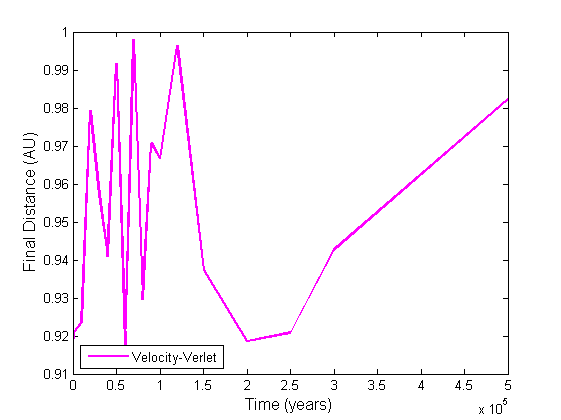
\includegraphics[width=1\linewidth]{Figures/test_distance_time_VV.png}
\end{minipage}%
\begin{minipage}{.5\textwidth}
  \centering
  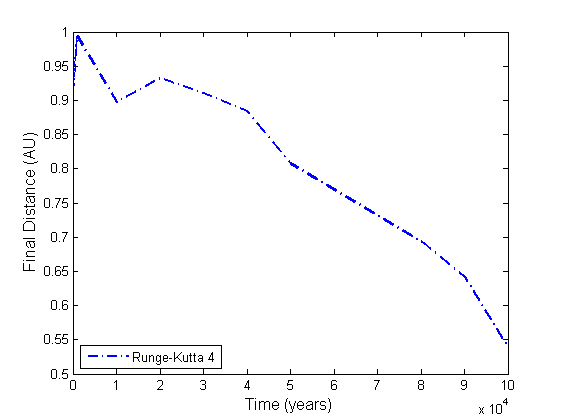
\includegraphics[width=1\linewidth]{Figures/test_distance_time_RK4.png}
\end{minipage}
\caption{
The final distance as a function of time with a time step length of 5 days for both the Velocity-Verlet and Runge-Kutta method with both the Earth and Sun moving relative to the frame of reference.
After $2.5\times 10^4$ years, the Earth continuously moves towards the Sun, in the Runge-Kutta method, whilst the distance between the Earth and Sun still fluctuates between 0.92 AU and 1 AU for the Velocity-Verlet method after $5\times 10^5$ years.  
}
\label{fig:SunEarthMarsTest2}
\end{figure}
When allowing for motion of both the Earth and the Sun relative to the frame of reference, both the Velocity-Verlet method and the forth order Runge-Kutta method show that the distance between the Earth-like body and the Sun-like body will fluctuate with time, which seems reasonable from the fact that Earth's orbit around the Sun is not circular but elliptical. 
From the Runge-Kutta method it is found that after approximately $2.5\times 10^4$ years the Earth will start moving rapidly towards the Sun, and after $10^5$ years the distance between the Sun-like object and the Earth-like object is only around $0.55$ AU. This is, however, not seen in the Velocity-Verlet method.
In the real solar system, the orbit of the Earth is in addition to the gravitational pull from the Sun also affected by the presence of the other planets. 
In the absence of these remaining planets and other objects in the solar system, the movement of the Earth-like object considered in this two-body system will, obviously, be different from the orbit known from astrophysics.
However, it is estimated that the absence of other objects in the solar system, will not cause this rapid motion of Earth and Sun towards each other after only in the order of $10,000$ years, and hence it is concluded that the rapid motion seen in the rightmost figure of \figref{fig:SunEarthMarsTest2} is due to instabilities in the fourth order Runge-Kutta method presented in \secref{sec:methodRK4}, yielding a greater stability in the Velocity-Verlet method than in the Runge-Kutta method for solving this two-body problem.

The table below shows the respective computational times for the fourth order Runge-Kutta method and the Velocity-Verlet method for computing the final position after 1 year using different time step length. 
\begin{table}[H]
\centering
\caption{
Computational time for the fourth order Runge-Kutta method and the Velocity-Verlet method for different time steps during 1 year.
}
\begin{center}
\begin{tabular}{ | c | c | c | }
  \hline			
  \# time steps  & Comp. time RK4 & Comp. time VV  
  \\ \hline
  1 & 6 & 2
  \\ \hline
  10 & 25 & 8
  \\ \hline
  $10^4$ & $8.4\times 10^3$ & $4.6\times 10^3$
  \\ \hline
  $10^6$ & $8.0\times 10^5$ & $3.6\times 10^5$
  \\ \hline
\end{tabular}
\end{center}
\label{tab:SunEarthMarsTest2}
\end{table}
From the table it is evident that the computational time of both the fourth order Runge-Kutta method and the Velocity-Verlet method is more or less proportional to the number of time steps.
Furthermore, the Velocity-Verlet method seems to be faster than the Runge-Kutta mthos for all investigated number of time steps. 
Together with the grater stability of the Velocity-Verlet method than the Runge-Kutta method, this yields that it is an advantage to use the Velocity-Verlet method to study this two-body system.  